%% Ankur Sinha

%% packages %%
% support for coloured text
\usepackage{color}
% IPA
\usepackage{tipa}
\usepackage[scale=2]{ccicons}
\usepackage{amssymb}
\usepackage{tikz}
\usetikzlibrary{mindmap, arrows.meta, positioning, arrows}
\usepackage{pgfplots}
% Define the colours we use for E and I in all graphs
\definecolor{SinhaBlueE}{HTML}{3b4cc0}
\definecolor{SinhaRedI}{HTML}{f7a789}
\pgfmathdeclarefunction{gaussnew}{4}{%nu, eta, eps, omega
  \pgfmathparse{(#1*((2*exp(-(((x-((#2+#3)/2))/((#2-#3)/(2*sqrt(-ln(#4/2)))))^2))) -#4))}%chktex 36
}
\usepackage{jneurosci}
\usepackage{subcaption}
\usepackage[T1]{fontenc}
\usepackage[utf8]{inputenc}
\usepackage[style=nature,backend=biber,autocite=footnote]{biblatex}
\addbibresource{/home/asinha/Documents/01_Readables/00_research_papers/bibliography/masterbib.bib}
% Use opensans
% \usepackage[default,scale=0.95]{opensans}
\usepackage[sfdefault]{roboto}
% for strike through
\usepackage[normalem]{ulem}
% links, urls, refs
\definecolor{links}{HTML}{2A1B81}
% Fedora blue for the theme
\definecolor{FedoraBlue}{HTML}{2A1B81}
\usepackage{hyperref}
\hypersetup{colorlinks,linkcolor=Green,urlcolor=links}
% graphics
\usepackage{graphicx}
% algorithm
\usepackage{algorithmic}
\usepackage{textcomp}
\usepackage{wrapfig}
\usepackage{textgreek}
\usepackage{euler}
\usepackage{csquotes}
\usepackage{tabularx}
\usepackage{booktabs}
% beamer theme
% use defaults for theme
\usetheme[numbering=fraction]{metropolis}
\usefonttheme[onlymath]{serif}
\setbeamerfont{footnote}{size=\tiny}
\setbeamerfont{caption}{size=\tiny}
\setbeamercolor{alerted text}{fg=Green}
\setbeamerfont{note page}{size=\small}

% Not needed in metropolis, but in general footnote citation fixes: https://tex.stackexchange.com/questions/44217/how-can-i-stop-footcite-from-hijacking-my-beamer-columns
% how to use multiple references to the same footnote: https://tex.stackexchange.com/questions/27763/beamer-multiple-references-to-the-same-footnote

% Disable footnoterule
\renewcommand{\footnoterule}{}

%% title %%
\title{Theory/modelling club!}
\subtitle{Structural plasticity and associative memory in balanced neural networks with spike-time dependent inhibitory plasticity}
\author[Ankur Sinha]{Ankur Sinha}
\date{02/06/2020}

%% document begins %%
\begin{document}


% title frame %%
\begin{frame}
  \titlepage{}
\end{frame}

%% Three slides for 5 minutes seems good
%% So, 30 slides at most for 50 minutes
\section{Context: what and why?}
\begin{frame}[c]{Peripheral lesions: large scale reorganisation in the brain}
  \begin{itemize}
    \item \fullcite{Rasmusson1982}
  \pause{}
  \scriptsize{
      \item \fullcite{Wall1984}
      \item \fullcite{Merzenich1984}
      \item \fullcite{Calford1988}
      \item \fullcite{Heinen1991}
      \item \fullcite{Rajan1993}
      }
  \end{itemize}
\end{frame}
\begin{frame}[c]{Imaging confirms structural plasticity in these experiments}
    \begin{itemize}
      \item \fullcite{DarianSmith1994}
        \pause{}
        \footnotesize{
      \item \fullcite{Florence1998}
      \item \fullcite{Keck2008}
      \item \fullcite{Keck2011}
      \item \fullcite{Marik2014}
      }
    \end{itemize}
\end{frame}
\begin{frame}[c]{Also confirms structural plasticity in the unlesioned adult brain}
    \begin{itemize}
      \item \fullcite{Holtmaat2005}
        \pause{}
        \footnotesize{
      \item \fullcite{Stettler2006}
      \item \fullcite{Marik2010}
      \item \fullcite{Chen2012}
      \item \fullcite{Villa2016}
      }
    \end{itemize}
\end{frame}
\begin{frame}[c]
  \frametitle{Example: Keck et al. 2008}
  \begin{figure}[h]
    \centering
    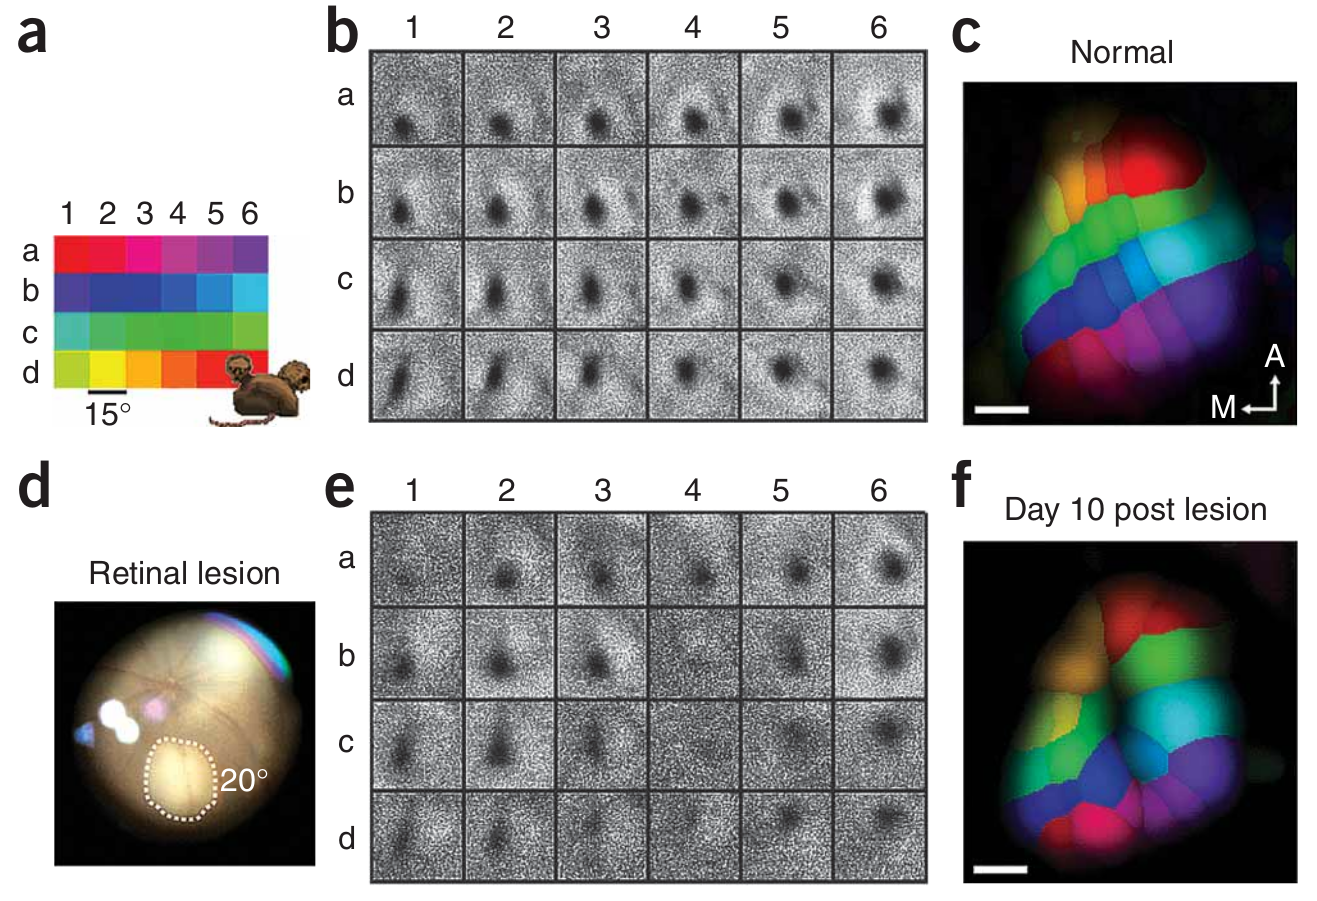
\includegraphics[width=0.8\linewidth]{99_images/keck-figure1}
  \end{figure}
  \footnotetext[1]{\fullcite{Keck2008}}
\end{frame}
\begin{frame}[c]
  \frametitle{Example: Keck et al. 2008: II}
  \begin{figure}[h]
    \centering
    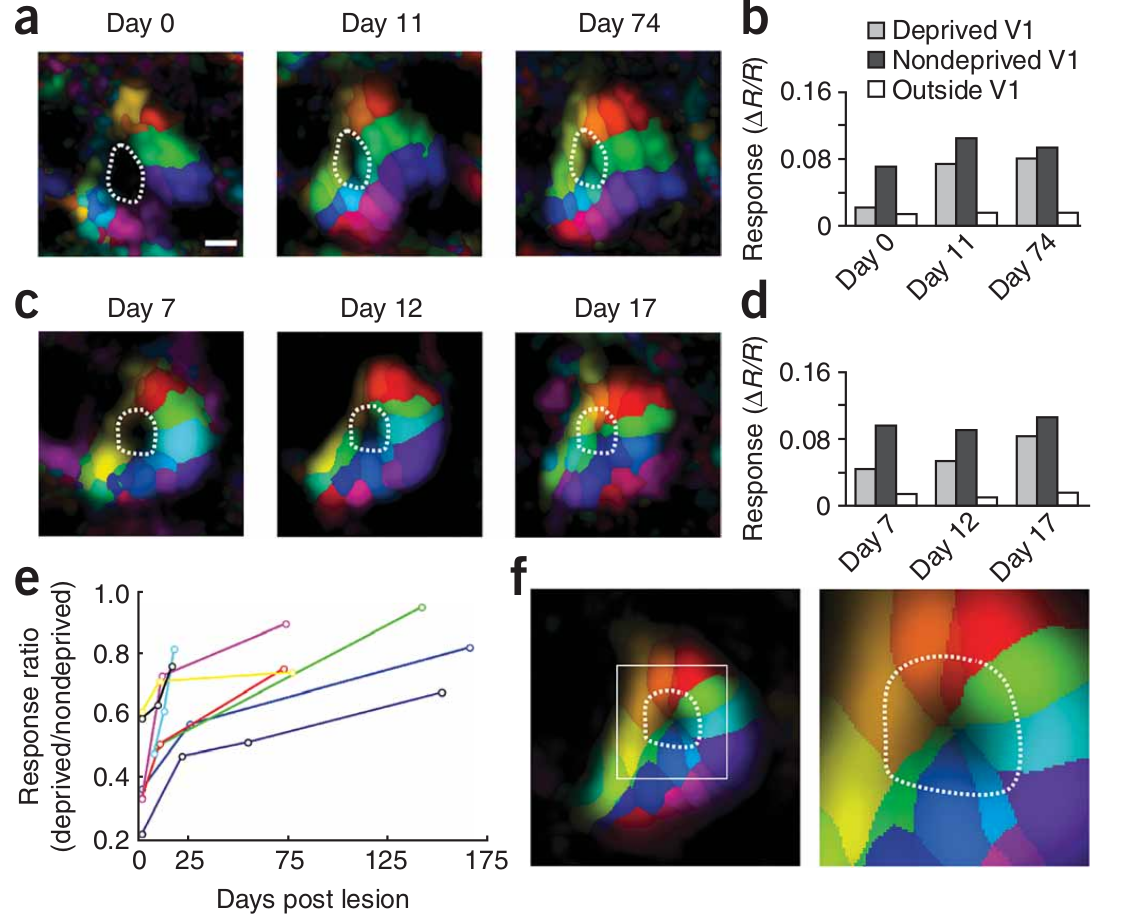
\includegraphics[width=0.8\linewidth]{99_images/keck-figure2}
  \end{figure}
  \footnotetext[1]{\fullcite{Keck2008}}
\end{frame}
\begin{frame}[c]
  \frametitle{Features of repair}
  \tiny{
\begin{table}[t]
  \centering
  \caption{Summary of review of literature on peripheral lesion experiments.}\label{tab:strp-lit-review}
  \begin{tabularx}{\textwidth}{XX}
    \toprule%
    \textbf{Observation} & \textbf{References} \\
    \midrule%
    \midrule%
    Recovery of neural response in deafferented regions. Inward restoration of activity in LPZ\@. & \textcite{Rasmusson1982,Merzenich1984,Calford1988,Heinen1991,Gilbert1992,Pons1991,Rajan1993,Florence1998}. \\
    \midrule%
    Sprouting of axons into the LPZ\@. & \textcite{DarianSmith1994,DarianSmith1995}. \\
    \midrule%
    Increase in density of dendritic spines on pyramidal cells in the LPZ\@. & \textcite{Keck2008}. \\
    \midrule%
    Ingrowth of excitatory axonal terminals to the LPZ, resulting in increase in density of axonal terminals in the region. & \textcite{Yamahachi2009}. \\
    \midrule%
    Loss in dendritic spines on inhibitory neurons receiving glutamatergic inputs in LPZ\@. & \textcite{Keck2011}. \\
    \midrule%
    Reduction in inhibitory boutons in LPZ\@. & \textcite{Keck2011}. \\
    \midrule%
    Disinhibition in LPZ after deafferentation. & \textcite{Chen2011,Keck2011}. \\
    \midrule%
    Outgrowth of inhibitory axons from the LPZ\@. & \textcite{Marik2010,Marik2014}. \\
    \bottomrule%
  \end{tabularx}
\end{table}
}

\end{frame}
\begin{frame}[c]
  \frametitle{Research question}
  How does repair by structural plasticity affect the function of the brain network?
\end{frame}
\section{How?}
\begin{frame}[c]
  \frametitle{Network dynamics during repair: Butz et al.}
  \begin{figure}[h]
    \centering
    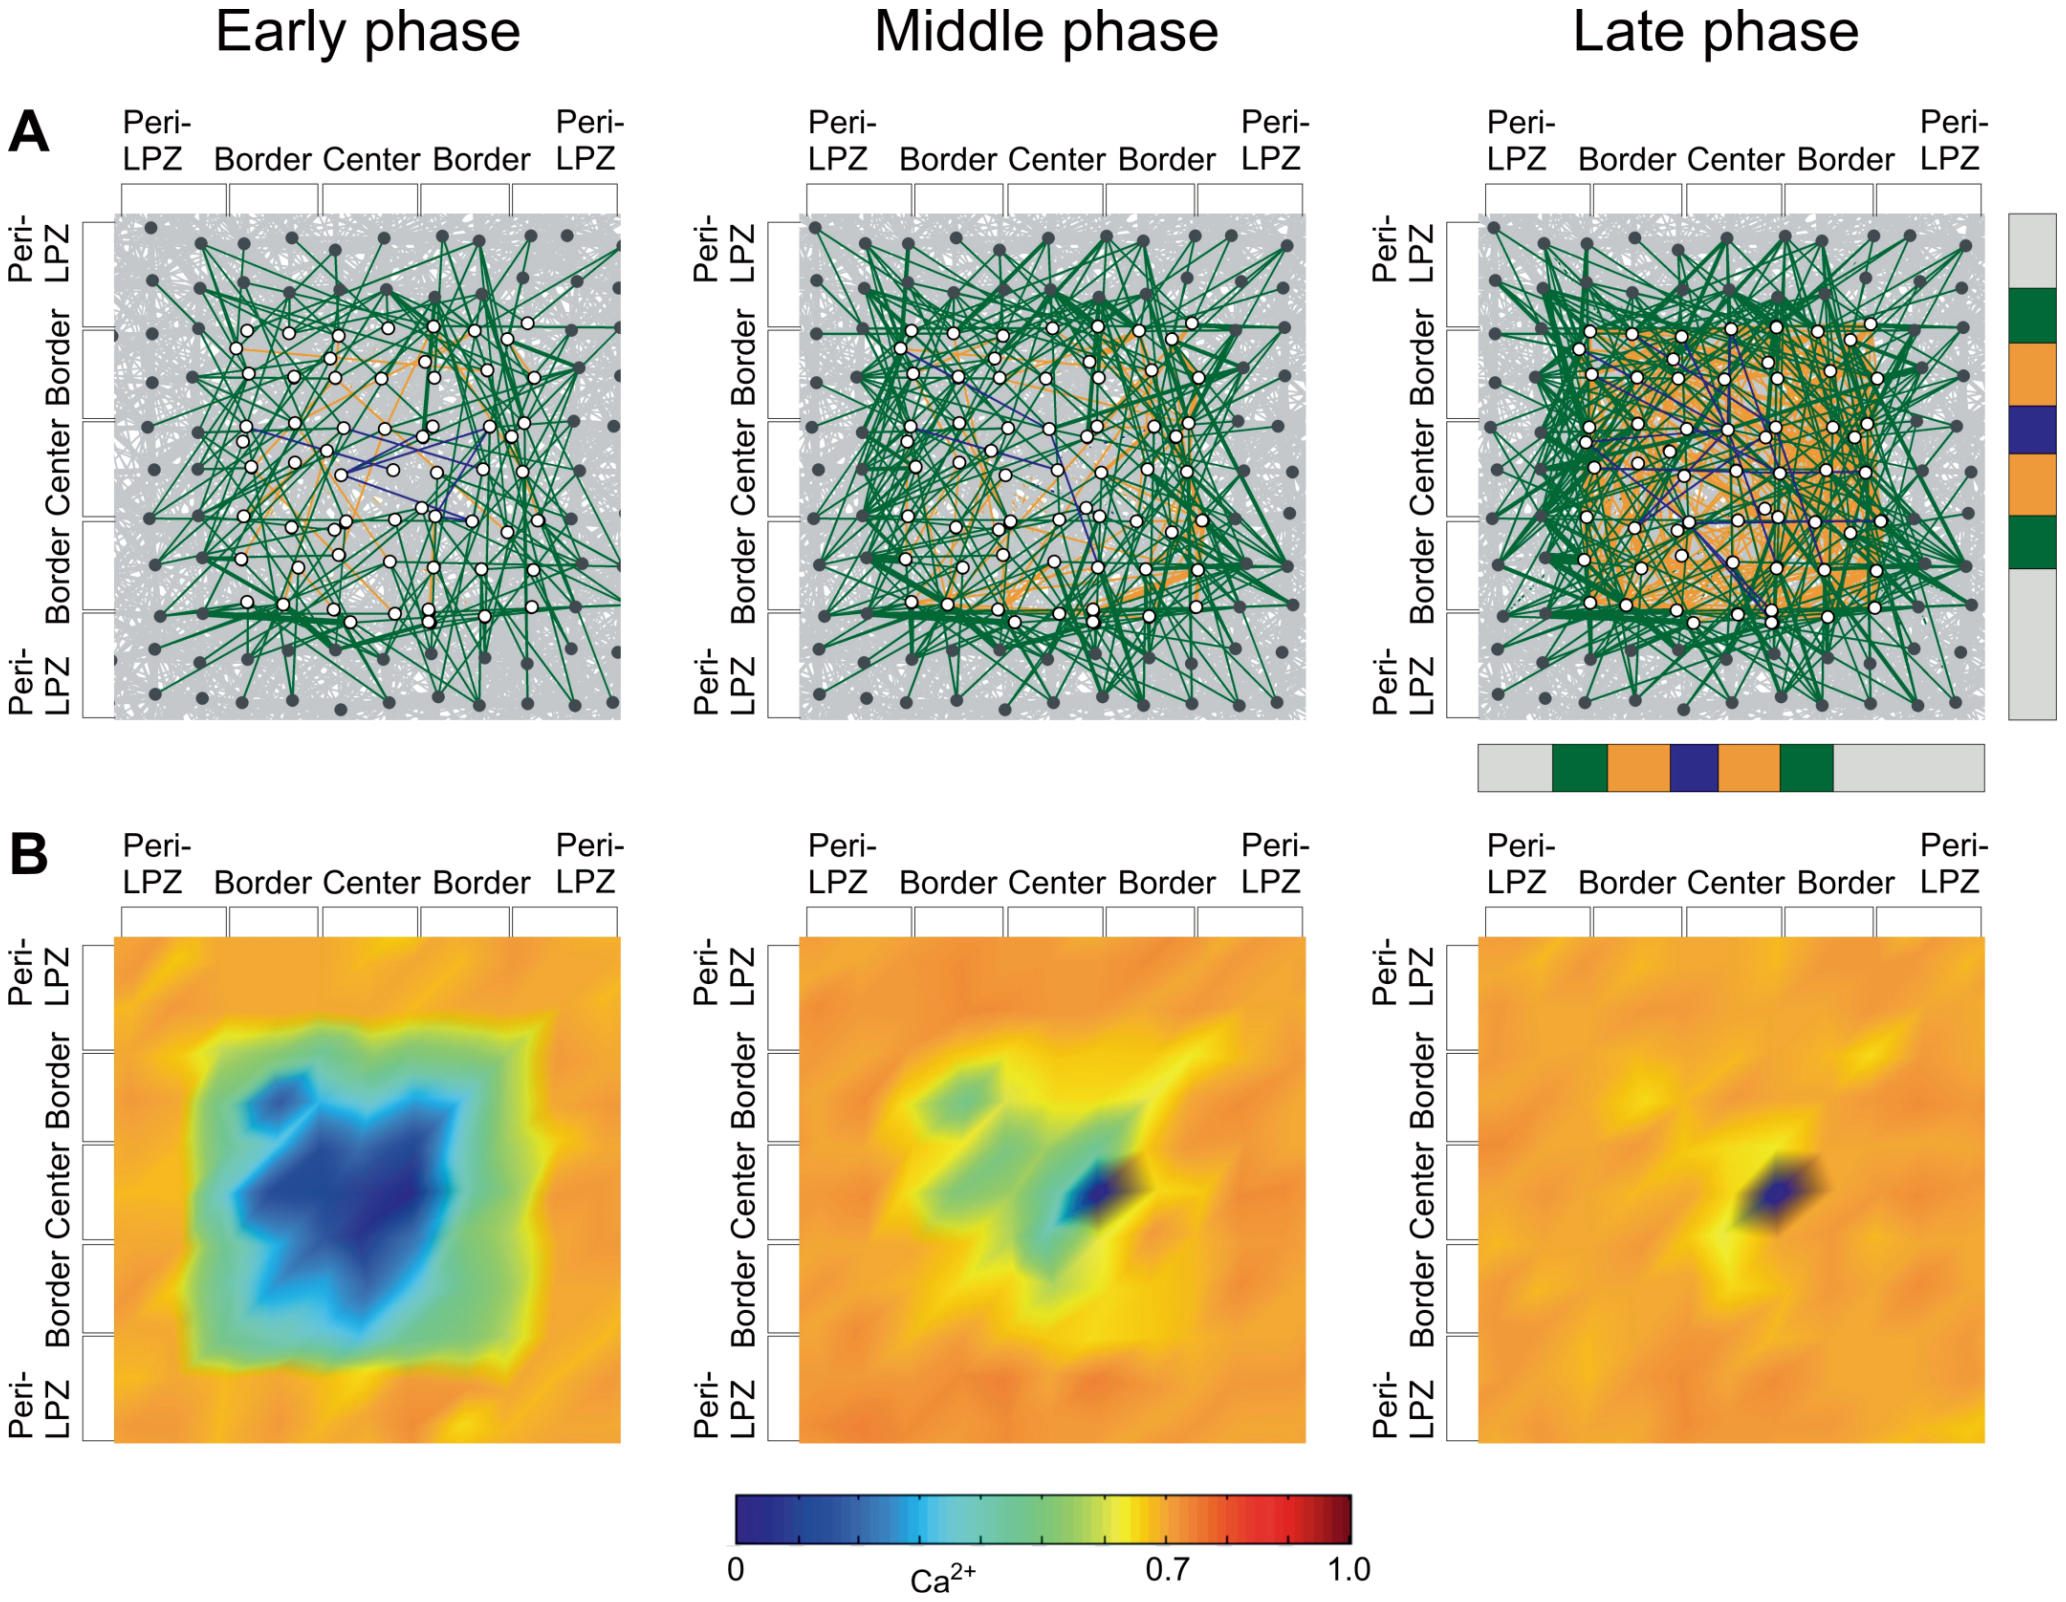
\includegraphics[width=0.8\linewidth]{99_images/butz3.png}
  \end{figure}
  \footnotetext[2]{\fullcite{Butz2013}}
\end{frame}
\begin{frame}[c]
  \frametitle{Butz2013: activity dependent homeostatic structural plasticity}
  \begin{columns}
    \begin{column}{0.5\textwidth}
      \begin{figure}[h]
        \centering
        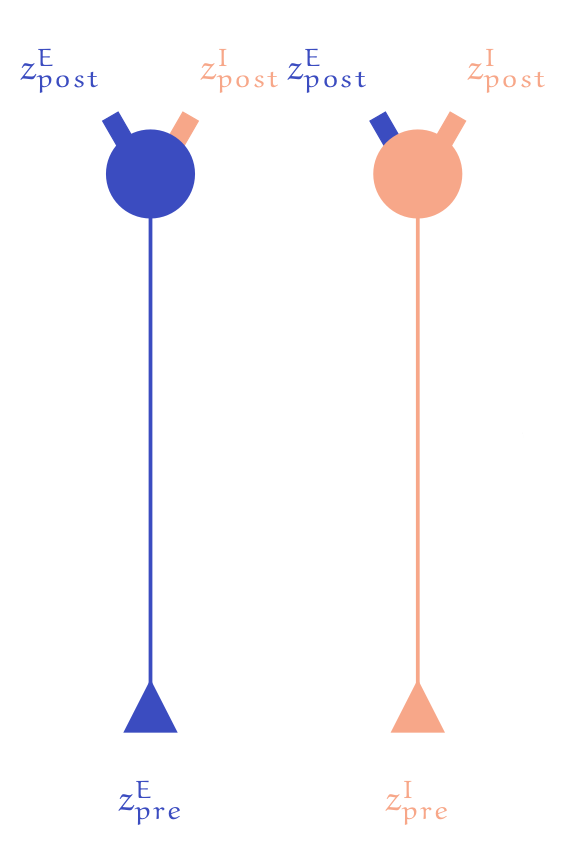
\includegraphics[width=0.8\linewidth]{99_images/neurons-strp}
      \end{figure}
    \end{column}
    \begin{column}{0.5\textwidth}
      \begin{figure}[h]
        \centering
        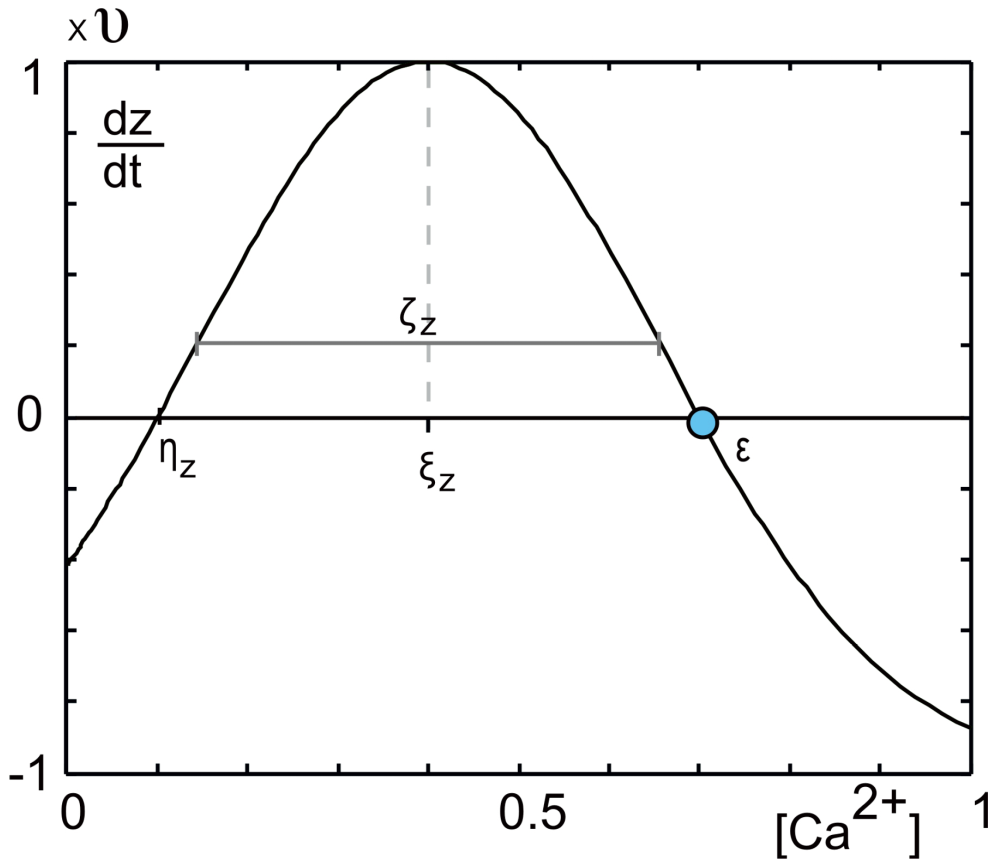
\includegraphics[width=0.8\linewidth]{99_images/growth-curve-general}
      \end{figure}
    \end{column}
  \end{columns}
  \footnotetext[2]{\fullcite{Butz2013}}
\end{frame}
\begin{frame}[c]
  \frametitle{Butz2013: activity dependent homeostatic structural plasticity}
  \begin{columns}
    \begin{column}{0.5\textwidth}
      \begin{figure}[h]
        \centering
        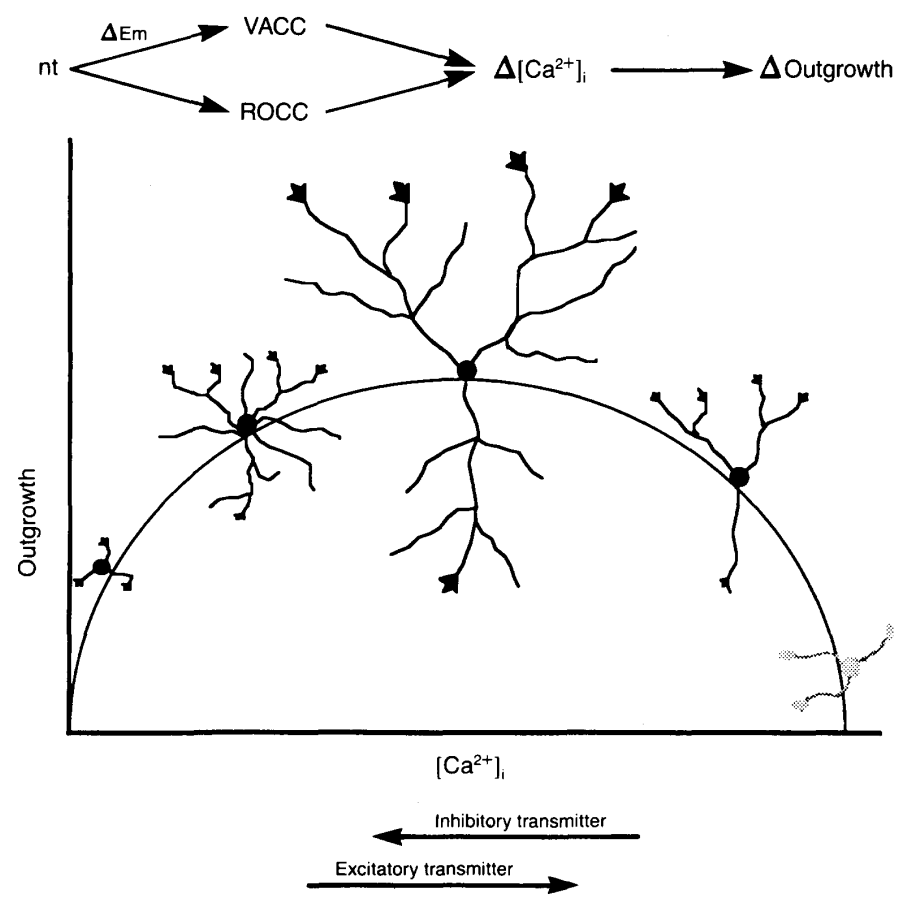
\includegraphics[width=0.8\linewidth]{99_images/lipton1989}
      \end{figure}
    \end{column}
    \begin{column}{0.5\textwidth}
      \begin{figure}[h]
        \centering
        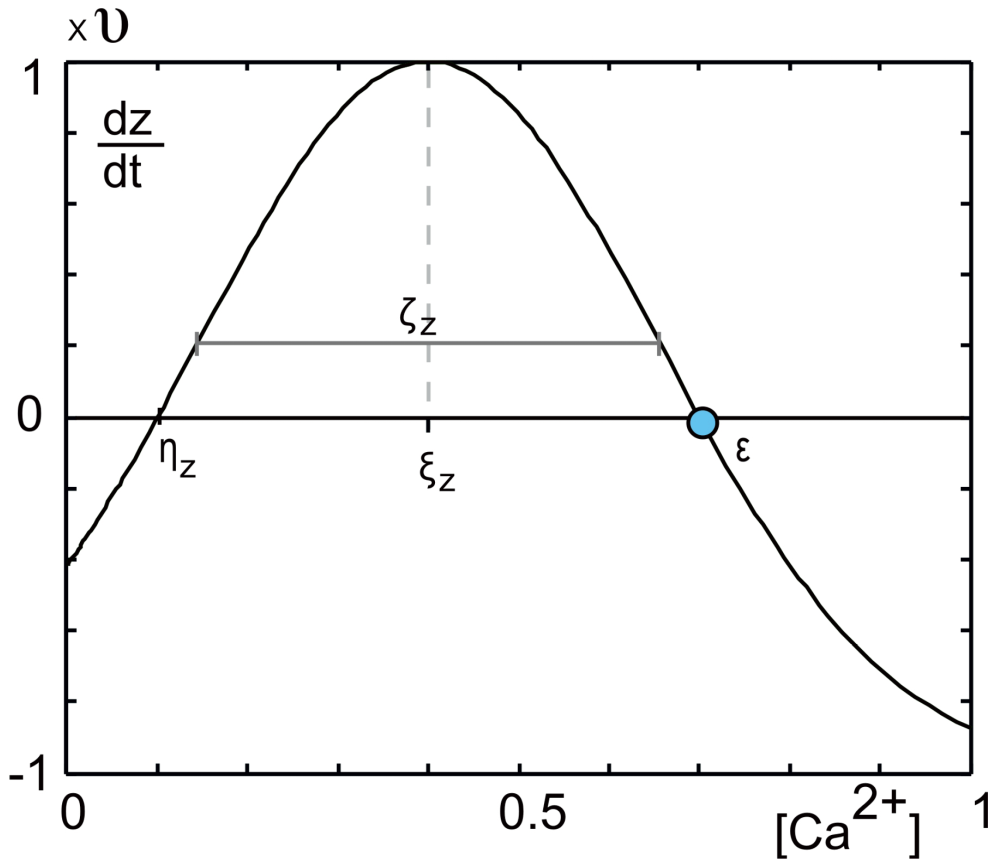
\includegraphics[width=0.8\linewidth]{99_images/growth-curve-general}
      \end{figure}
    \end{column}
  \end{columns}
  \footnotetext[2]{\fullcite{Butz2013}}
  \footnotetext[3]{\fullcite{Lipton1989}}
\end{frame}
\begin{frame}[c]
  \frametitle{Re-implementation/investigation of Butz et al.'s model}
  \tiny{
\begin{table}[t]
  \centering
  \caption{Summary of experimental observations reproduced in the model proposed by \textcite{Butz2013}.}\label{tab:butz-results}
  \begin{tabularx}{\textwidth}{XX}
    \toprule%
    \textbf{Experimental observation} & \textbf{Reproduced} \\
    \midrule%
    \midrule%
    Gradual inward restoration of activity in LPZ\@. & Yes. \\
    \midrule%
    Sprouting of axons into the LPZ\@. & Yes. \\
    \midrule%
    Increase in density of dendritic spines on pyramidal cells in the LPZ\@. & Yes. \\
    \midrule%
    Ingrowth of excitatory axonal terminals to the LPZ, resulting in increase in density of axonal terminals in the region. & Yes. \\
    \midrule%
    Loss in dendritic spines on inhibitory neurons receiving glutamatergic inputs in LPZ\@. & No---increase of all synaptic elements in neurons of LPZ\@. \\
    \midrule%
    Reduction in inhibitory boutons in LPZ\@. & No---increase in inhibitory axonal contacts also.  \\
    \midrule%
    Disinhibition in LPZ after deafferentation. & No. \\
    \midrule%
    Outgrowth of inhibitory axons from the LPZ\@. & No---ingrowth of inhibitory axons also. \\
    \bottomrule%
  \end{tabularx}
\end{table}
}

\end{frame}
\begin{frame}[c]
  \frametitle{Proxy for network function: associative memory storage}
  \begin{figure}[h]
    \centering
    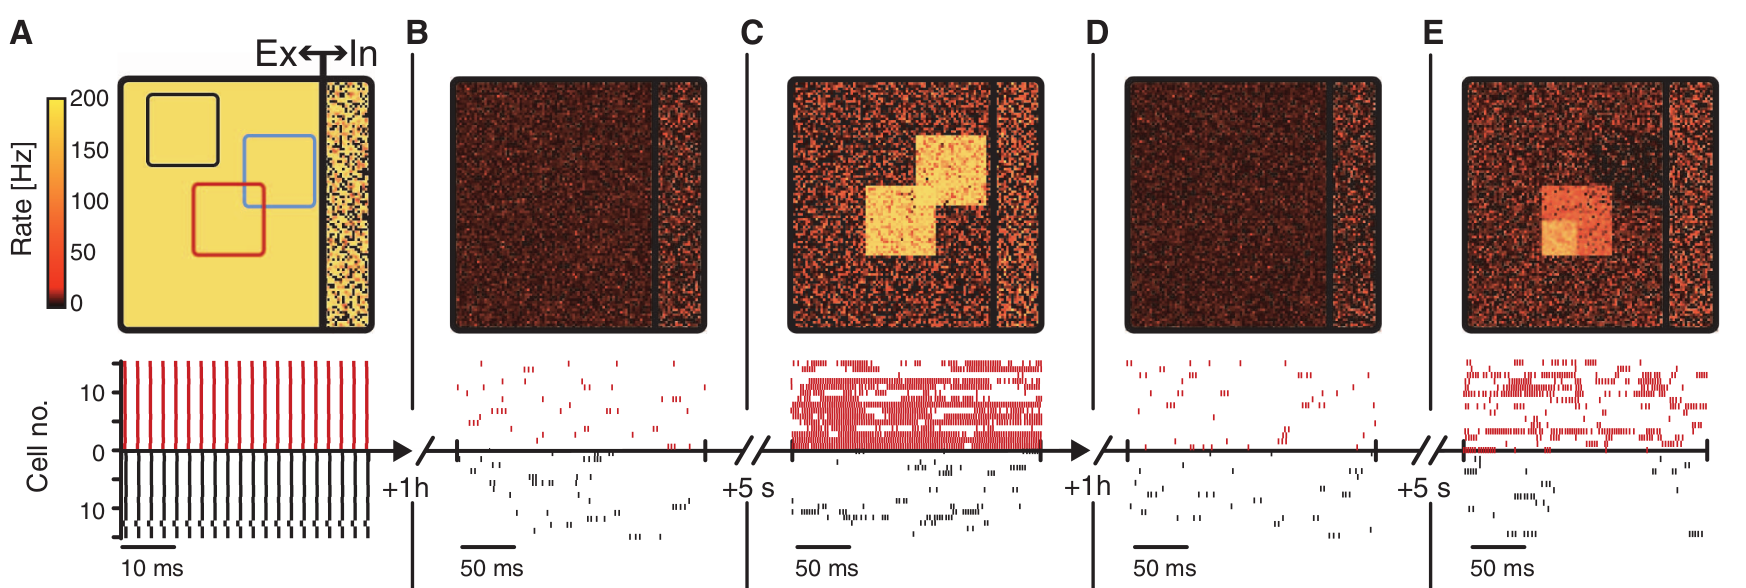
\includegraphics[width=\linewidth]{99_images/vogels-figure4}
  \end{figure}
  \footnotetext[4]{\fullcite{Vogels2011}}
\end{frame}
\begin{frame}[c]
  \frametitle{Re-implementation/verification of associative memory model}
  \begin{figure}[htpb]
  \begin{subfigure}[h]{0.3\textwidth}
    \resizebox{1.2\textwidth}{!}{% GNUPLOT: LaTeX picture with Postscript
\begingroup
  \makeatletter
  \providecommand\color[2][]{%
    \GenericError{(gnuplot) \space\space\space\@spaces}{%
      Package color not loaded in conjunction with
      terminal option `colourtext'%
    }{See the gnuplot documentation for explanation.%
    }{Either use `blacktext' in gnuplot or load the package
      color.sty in LaTeX.}%
    \renewcommand\color[2][]{}%
  }%
  \providecommand\includegraphics[2][]{%
    \GenericError{(gnuplot) \space\space\space\@spaces}{%
      Package graphicx or graphics not loaded%
    }{See the gnuplot documentation for explanation.%
    }{The gnuplot epslatex terminal needs graphicx.sty or graphics.sty.}%
    \renewcommand\includegraphics[2][]{}%
  }%
  \providecommand\rotatebox[2]{#2}%
  \@ifundefined{ifGPcolor}{%
    \newif\ifGPcolor{}
    \GPcolortrue{}
  }{}%
  \@ifundefined{ifGPblacktext}{%
    \newif\ifGPblacktext{}
    \GPblacktextfalse{}
  }{}%
  % define a \g@addto@macro without @ in the name:
  \let\gplgaddtomacro\g@addto@macro{}
  % define empty templates for all commands taking text:
  \gdef\gplbacktext{}%
  \gdef\gplfronttext{}%
  \makeatother
  \ifGPblacktext{}
    % no textcolor at all
    \def\colorrgb#1{}%
    \def\colorgray#1{}%
  \else
    % gray or color?
    \ifGPcolor{}
      \def\colorrgb#1{\color[rgb]{#1}}%
      \def\colorgray#1{\color[gray]{#1}}%
      \expandafter\def\csname LTw\endcsname{\color{white}}%
      \expandafter\def\csname LTb\endcsname{\color{black}}%
      \expandafter\def\csname LTa\endcsname{\color{black}}%
      \expandafter\def\csname LT0\endcsname{\color[rgb]{1,0,0}}%
      \expandafter\def\csname LT1\endcsname{\color[rgb]{0,1,0}}%
      \expandafter\def\csname LT2\endcsname{\color[rgb]{0,0,1}}%
      \expandafter\def\csname LT3\endcsname{\color[rgb]{1,0,1}}%
      \expandafter\def\csname LT4\endcsname{\color[rgb]{0,1,1}}%
      \expandafter\def\csname LT5\endcsname{\color[rgb]{1,1,0}}%
      \expandafter\def\csname LT6\endcsname{\color[rgb]{0,0,0}}%
      \expandafter\def\csname LT7\endcsname{\color[rgb]{1,0.3,0}}%
      \expandafter\def\csname LT8\endcsname{\color[rgb]{0.5,0.5,0.5}}%
    \else
      % gray
      \def\colorrgb#1{\color{black}}%
      \def\colorgray#1{\color[gray]{#1}}%
      \expandafter\def\csname LTw\endcsname{\color{white}}%
      \expandafter\def\csname LTb\endcsname{\color{black}}%
      \expandafter\def\csname LTa\endcsname{\color{black}}%
      \expandafter\def\csname LT0\endcsname{\color{black}}%
      \expandafter\def\csname LT1\endcsname{\color{black}}%
      \expandafter\def\csname LT2\endcsname{\color{black}}%
      \expandafter\def\csname LT3\endcsname{\color{black}}%
      \expandafter\def\csname LT4\endcsname{\color{black}}%
      \expandafter\def\csname LT5\endcsname{\color{black}}%
      \expandafter\def\csname LT6\endcsname{\color{black}}%
      \expandafter\def\csname LT7\endcsname{\color{black}}%
      \expandafter\def\csname LT8\endcsname{\color{black}}%
    \fi
  \fi
    \setlength{\unitlength}{0.0500bp}%
    \ifx\gptboxheight\undefined%
      \newlength{\gptboxheight}%
      \newlength{\gptboxwidth}%
      \newsavebox{\gptboxtext}%
    \fi%
    \setlength{\fboxrule}{0.5pt}%
    \setlength{\fboxsep}{1pt}%
\begin{picture}(7200.00,5040.00)%
    \gplgaddtomacro\gplbacktext{%
      \csname LTb\endcsname%
      \put(900,4400){\makebox(0,0)[r]{\strut{}\(100\)}}%
      \put(900,400){\makebox(0,0){\strut{}\(0\)}}%
      \put(4150,400){\makebox(0,0){\strut{}\(80\)}}%
      \put(5000,400){\makebox(0,0){\strut{}\(100\)}}%
    }%
    \gplgaddtomacro\gplfronttext{%
      \csname LTb\endcsname%
      \put(5500,2500){\rotatebox{-270}{\makebox(0,0){\strut{}Firing rate (Hz)}}}%
      \put(800,2539){\rotatebox{-270}{\makebox(0,0){\strut{}Neurons}}}%
      \put(3000,400){\makebox(0,0){\strut{}Neurons}}%
      \csname LTb\endcsname%
      \put(5700,4400){\makebox(0,0)[r]{\strut{}\(140\)}}%
      \csname LTb\endcsname%
      \put(5450,600){\makebox(0,0)[r]{\strut{}\(0\)}}%
    }%
    \gplbacktext
    \put(1000,600){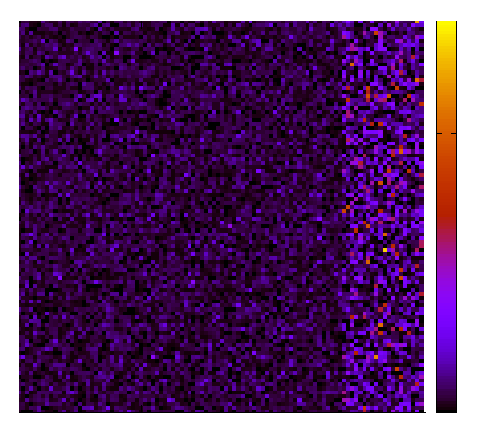
\includegraphics{99_images/B-ratematrix-notext}}%
    \gplfronttext
  \end{picture}%
\endgroup
}
  \end{subfigure}
  \begin{subfigure}[h]{0.3\textwidth}
    \resizebox{1.2\textwidth}{!}{% GNUPLOT: LaTeX picture with Postscript
\begingroup
  \makeatletter
  \providecommand\color[2][]{%
    \GenericError{(gnuplot) \space\space\space\@spaces}{%
      Package color not loaded in conjunction with
      terminal option `colourtext'%
    }{See the gnuplot documentation for explanation.%
    }{Either use `blacktext' in gnuplot or load the package
      color.sty in LaTeX.}%
    \renewcommand\color[2][]{}%
  }%
  \providecommand\includegraphics[2][]{%
    \GenericError{(gnuplot) \space\space\space\@spaces}{%
      Package graphicx or graphics not loaded%
    }{See the gnuplot documentation for explanation.%
    }{The gnuplot epslatex terminal needs graphicx.sty or graphics.sty.}%
    \renewcommand\includegraphics[2][]{}%
  }%
  \providecommand\rotatebox[2]{#2}%
  \@ifundefined{ifGPcolor}{%
    \newif\ifGPcolor{}
    \GPcolortrue{}
  }{}%
  \@ifundefined{ifGPblacktext}{%
    \newif\ifGPblacktext{}
    \GPblacktextfalse{}
  }{}%
  % define a \g@addto@macro without @ in the name:
  \let\gplgaddtomacro\g@addto@macro{}
  % define empty templates for all commands taking text:
  \gdef\gplbacktext{}%
  \gdef\gplfronttext{}%
  \makeatother
  \ifGPblacktext{}
    % no textcolor at all
    \def\colorrgb#1{}%
    \def\colorgray#1{}%
  \else
    % gray or color?
    \ifGPcolor{}
      \def\colorrgb#1{\color[rgb]{#1}}%
      \def\colorgray#1{\color[gray]{#1}}%
      \expandafter\def\csname LTw\endcsname{\color{white}}%
      \expandafter\def\csname LTb\endcsname{\color{black}}%
      \expandafter\def\csname LTa\endcsname{\color{black}}%
      \expandafter\def\csname LT0\endcsname{\color[rgb]{1,0,0}}%
      \expandafter\def\csname LT1\endcsname{\color[rgb]{0,1,0}}%
      \expandafter\def\csname LT2\endcsname{\color[rgb]{0,0,1}}%
      \expandafter\def\csname LT3\endcsname{\color[rgb]{1,0,1}}%
      \expandafter\def\csname LT4\endcsname{\color[rgb]{0,1,1}}%
      \expandafter\def\csname LT5\endcsname{\color[rgb]{1,1,0}}%
      \expandafter\def\csname LT6\endcsname{\color[rgb]{0,0,0}}%
      \expandafter\def\csname LT7\endcsname{\color[rgb]{1,0.3,0}}%
      \expandafter\def\csname LT8\endcsname{\color[rgb]{0.5,0.5,0.5}}%
    \else
      % gray
      \def\colorrgb#1{\color{black}}%
      \def\colorgray#1{\color[gray]{#1}}%
      \expandafter\def\csname LTw\endcsname{\color{white}}%
      \expandafter\def\csname LTb\endcsname{\color{black}}%
      \expandafter\def\csname LTa\endcsname{\color{black}}%
      \expandafter\def\csname LT0\endcsname{\color{black}}%
      \expandafter\def\csname LT1\endcsname{\color{black}}%
      \expandafter\def\csname LT2\endcsname{\color{black}}%
      \expandafter\def\csname LT3\endcsname{\color{black}}%
      \expandafter\def\csname LT4\endcsname{\color{black}}%
      \expandafter\def\csname LT5\endcsname{\color{black}}%
      \expandafter\def\csname LT6\endcsname{\color{black}}%
      \expandafter\def\csname LT7\endcsname{\color{black}}%
      \expandafter\def\csname LT8\endcsname{\color{black}}%
    \fi
  \fi
    \setlength{\unitlength}{0.0500bp}%
    \ifx\gptboxheight\undefined%
      \newlength{\gptboxheight}%
      \newlength{\gptboxwidth}%
      \newsavebox{\gptboxtext}%
    \fi%
    \setlength{\fboxrule}{0.5pt}%
    \setlength{\fboxsep}{1pt}%
\begin{picture}(7200.00,5040.00)%
    \gplgaddtomacro\gplbacktext{%
      \csname LTb\endcsname%
      \put(900,4400){\makebox(0,0)[r]{\strut{}\(100\)}}%
      \put(900,400){\makebox(0,0){\strut{}\(0\)}}%
      \put(4150,400){\makebox(0,0){\strut{}\(80\)}}%
      \put(5000,400){\makebox(0,0){\strut{}\(100\)}}%
    }%
    \gplgaddtomacro\gplfronttext{%
      \csname LTb\endcsname%
      \put(5500,2500){\rotatebox{-270}{\makebox(0,0){\strut{}Firing rate (Hz)}}}%
      \put(800,2539){\rotatebox{-270}{\makebox(0,0){\strut{}Neurons}}}%
      \put(3000,400){\makebox(0,0){\strut{}Neurons}}%
      \csname LTb\endcsname%
      \put(5700,4400){\makebox(0,0)[r]{\strut{}\(140\)}}%
      \csname LTb\endcsname%
      \put(5450,600){\makebox(0,0)[r]{\strut{}\(0\)}}%
    }%
    \gplbacktext
    \put(1000,600){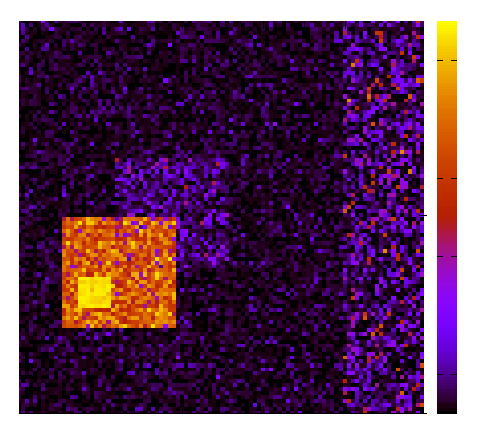
\includegraphics{99_images/C-ratematrix-notext}}%
    \gplfronttext
  \end{picture}%
\endgroup
}
  \end{subfigure}
  \begin{subfigure}[c]{0.3\textwidth}
    \resizebox{1.2\textwidth}{!}{% GNUPLOT: LaTeX picture with Postscript
\begingroup
  \makeatletter
  \providecommand\color[2][]{%
    \GenericError{(gnuplot) \space\space\space\@spaces}{%
      Package color not loaded in conjunction with
      terminal option `colourtext'%
    }{See the gnuplot documentation for explanation.%
    }{Either use `blacktext' in gnuplot or load the package
      color.sty in LaTeX.}%
    \renewcommand\color[2][]{}%
  }%
  \providecommand\includegraphics[2][]{%
    \GenericError{(gnuplot) \space\space\space\@spaces}{%
      Package graphicx or graphics not loaded%
    }{See the gnuplot documentation for explanation.%
    }{The gnuplot epslatex terminal needs graphicx.sty or graphics.sty.}%
    \renewcommand\includegraphics[2][]{}%
  }%
  \providecommand\rotatebox[2]{#2}%
  \@ifundefined{ifGPcolor}{%
    \newif\ifGPcolor{}
    \GPcolortrue{}
  }{}%
  \@ifundefined{ifGPblacktext}{%
    \newif\ifGPblacktext{}
    \GPblacktextfalse{}
  }{}%
  % define a \g@addto@macro without @ in the name:
  \let\gplgaddtomacro\g@addto@macro{}
  % define empty templates for all commands taking text:
  \gdef\gplbacktext{}%
  \gdef\gplfronttext{}%
  \makeatother
  \ifGPblacktext{}
    % no textcolor at all
    \def\colorrgb#1{}%
    \def\colorgray#1{}%
  \else
    % gray or color?
    \ifGPcolor{}
      \def\colorrgb#1{\color[rgb]{#1}}%
      \def\colorgray#1{\color[gray]{#1}}%
      \expandafter\def\csname LTw\endcsname{\color{white}}%
      \expandafter\def\csname LTb\endcsname{\color{black}}%
      \expandafter\def\csname LTa\endcsname{\color{black}}%
      \expandafter\def\csname LT0\endcsname{\color[rgb]{1,0,0}}%
      \expandafter\def\csname LT1\endcsname{\color[rgb]{0,1,0}}%
      \expandafter\def\csname LT2\endcsname{\color[rgb]{0,0,1}}%
      \expandafter\def\csname LT3\endcsname{\color[rgb]{1,0,1}}%
      \expandafter\def\csname LT4\endcsname{\color[rgb]{0,1,1}}%
      \expandafter\def\csname LT5\endcsname{\color[rgb]{1,1,0}}%
      \expandafter\def\csname LT6\endcsname{\color[rgb]{0,0,0}}%
      \expandafter\def\csname LT7\endcsname{\color[rgb]{1,0.3,0}}%
      \expandafter\def\csname LT8\endcsname{\color[rgb]{0.5,0.5,0.5}}%
    \else
      % gray
      \def\colorrgb#1{\color{black}}%
      \def\colorgray#1{\color[gray]{#1}}%
      \expandafter\def\csname LTw\endcsname{\color{white}}%
      \expandafter\def\csname LTb\endcsname{\color{black}}%
      \expandafter\def\csname LTa\endcsname{\color{black}}%
      \expandafter\def\csname LT0\endcsname{\color{black}}%
      \expandafter\def\csname LT1\endcsname{\color{black}}%
      \expandafter\def\csname LT2\endcsname{\color{black}}%
      \expandafter\def\csname LT3\endcsname{\color{black}}%
      \expandafter\def\csname LT4\endcsname{\color{black}}%
      \expandafter\def\csname LT5\endcsname{\color{black}}%
      \expandafter\def\csname LT6\endcsname{\color{black}}%
      \expandafter\def\csname LT7\endcsname{\color{black}}%
      \expandafter\def\csname LT8\endcsname{\color{black}}%
    \fi
  \fi
    \setlength{\unitlength}{0.0500bp}%
    \ifx\gptboxheight\undefined%
      \newlength{\gptboxheight}%
      \newlength{\gptboxwidth}%
      \newsavebox{\gptboxtext}%
    \fi%
    \setlength{\fboxrule}{0.5pt}%
    \setlength{\fboxsep}{1pt}%
\begin{picture}(7200.00,5040.00)%
    \gplgaddtomacro\gplbacktext{%
      \csname LTb\endcsname%
      \put(900,4400){\makebox(0,0)[r]{\strut{}\(100\)}}%
      \put(900,400){\makebox(0,0){\strut{}\(0\)}}%
      \put(4150,400){\makebox(0,0){\strut{}\(80\)}}%
      \put(5000,400){\makebox(0,0){\strut{}\(100\)}}%
    }%
    \gplgaddtomacro\gplfronttext{%
      \csname LTb\endcsname%
      \put(5500,2500){\rotatebox{-270}{\makebox(0,0){\strut{}Firing rate (Hz)}}}%
      \put(800,2539){\rotatebox{-270}{\makebox(0,0){\strut{}Neurons}}}%
      \put(3000,400){\makebox(0,0){\strut{}Neurons}}%
      \csname LTb\endcsname%
      \put(5700,4400){\makebox(0,0)[r]{\strut{}\(140\)}}%
      \csname LTb\endcsname%
      \put(5450,600){\makebox(0,0)[r]{\strut{}\(0\)}}%
    }%
    \gplbacktext
    \put(1000,600){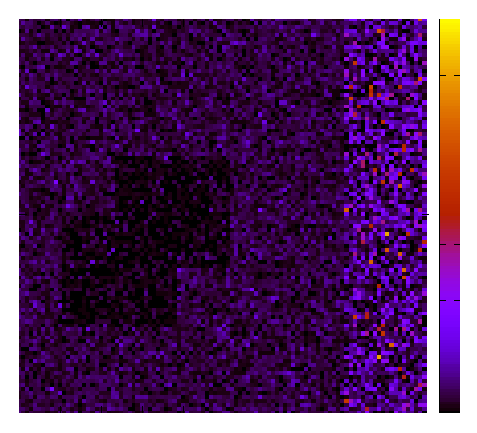
\includegraphics{99_images/D-ratematrix-notext}}%
    \gplfronttext
  \end{picture}%
\endgroup
}
  \end{subfigure}
  \end{figure}
\end{frame}
\begin{frame}[c]
  \frametitle{Expected research path}
  Apply Butz et al.'s model of structural plasticity to the Vogels-Sprekeler's cortical model, store associative memories, measure performance before, during, after repair.
\end{frame}
\begin{frame}[c]
  \frametitle{Model schematic}
  \begin{figure}[h]
    \centering
    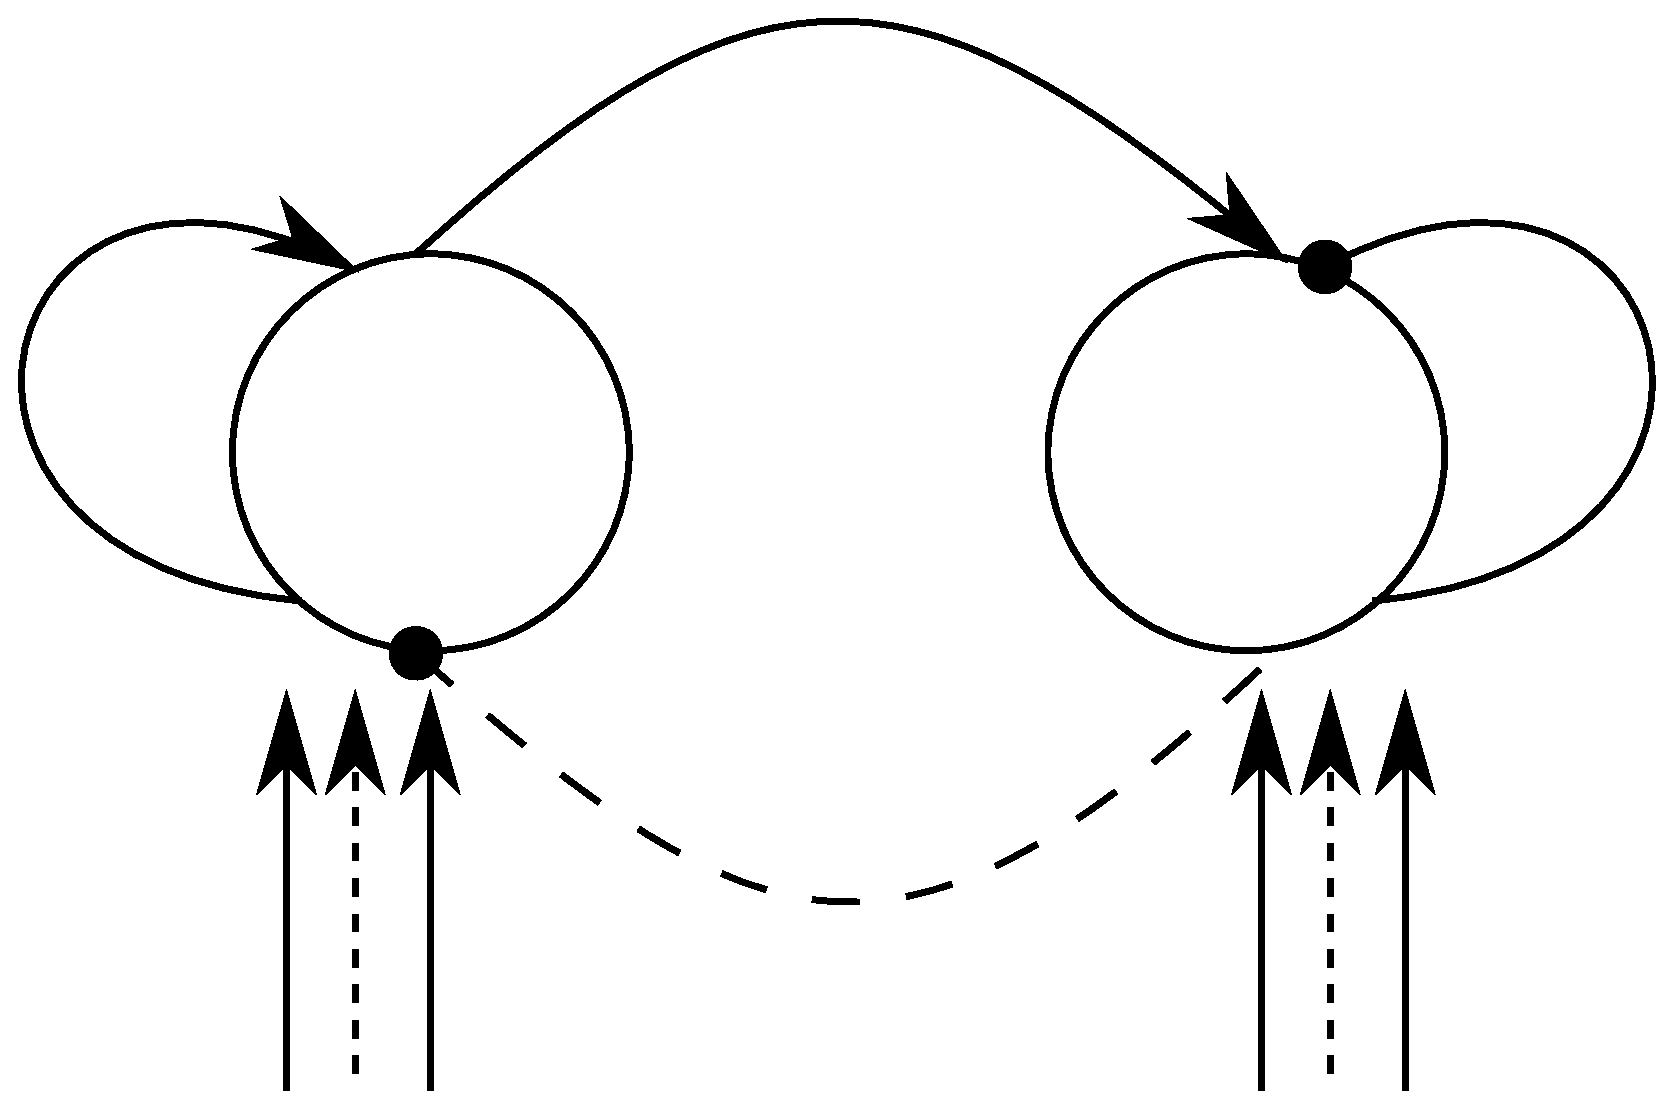
\includegraphics[width=0.8\linewidth]{99_images/schematic}
  \end{figure}
\end{frame}
\begin{frame}[c]
  \frametitle{Simulation protocol}
  \begin{figure}[h]
    \centering
    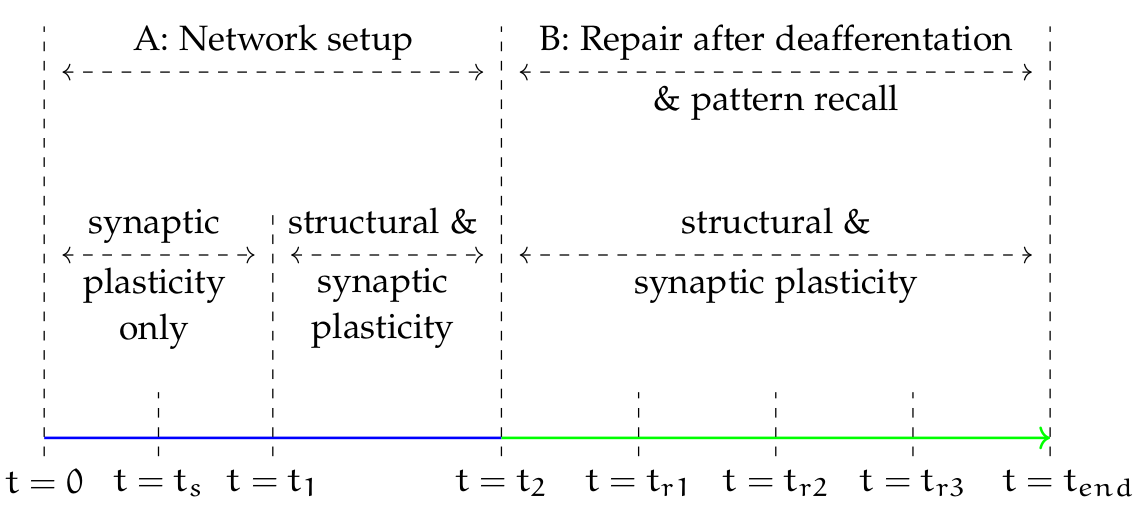
\includegraphics[width=0.8\linewidth]{99_images/recall-protocol}
  \end{figure}
\end{frame}
\begin{frame}[c]
  \frametitle{Effect of deafferentation on cortical model}
  \begin{figure}[h]
    \centering
    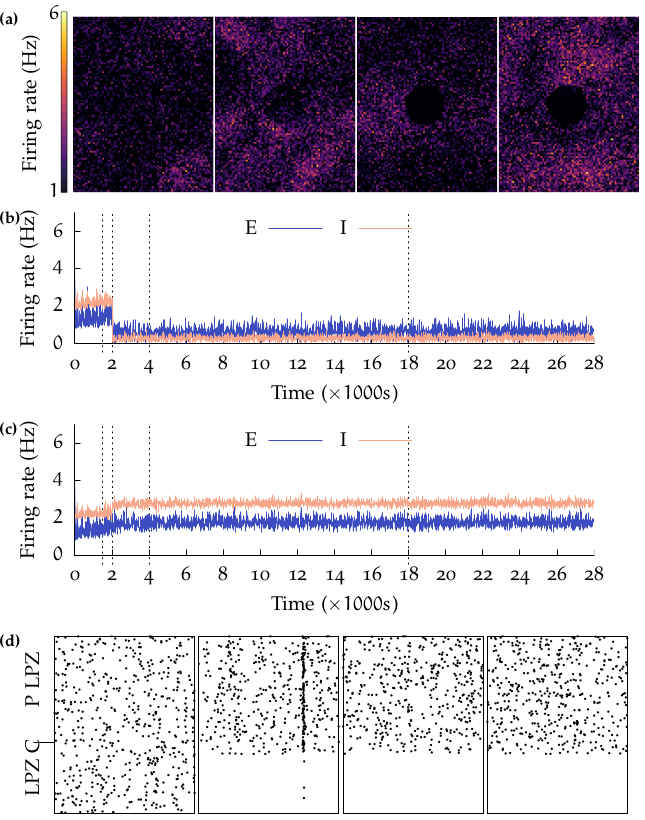
\includegraphics[width=0.5\linewidth]{99_images/deaff-only}
  \end{figure}
\end{frame}
\begin{frame}[c]
  \frametitle{Rejection of Butz et al.'s growth curve hypothesis}
  If Butz et al.'s single growth curve for all neurites is correct, the increase in activity outside the LPZ  as a result of deafferentation will cause:
  \begin{itemize}
    \item retraction of excitatory pre-synaptic elements outside the LPZ,
    \item retraction of inhibitory post-synaptic elements outside the LPZ\@.
  \end{itemize}
\end{frame}
\section{Results}
\begin{frame}[c]
  \frametitle{New model of peripheral lesioning and repair in cortical network}
  \begin{figure}[h]
    \centering
    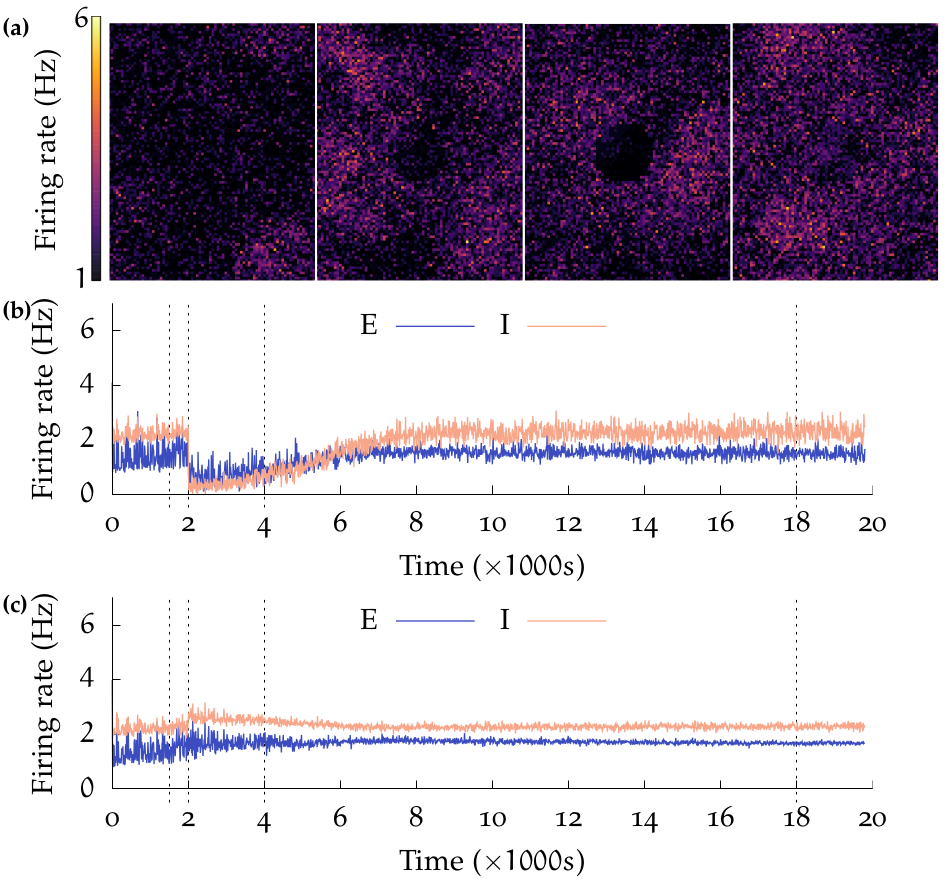
\includegraphics[width=0.5\linewidth]{99_images/deaff-repair}
  \end{figure}
  \footnotetext[5]{\fullcite{Sinha2019}}
\end{frame}
\begin{frame}[c]
  \frametitle{New growth curves for post-synaptic neurites}
  \begin{figure}[h]
    \centering
    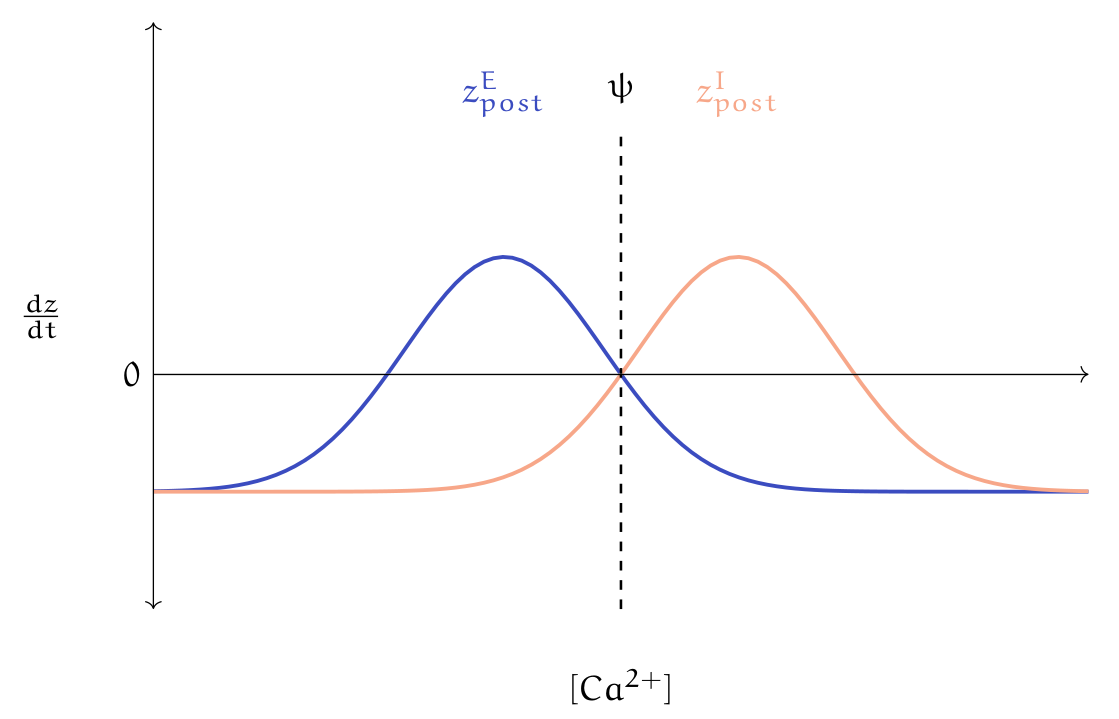
\includegraphics[width=0.6\linewidth]{99_images/growth-post}
  \end{figure}
\end{frame}
\begin{frame}[c]
  \frametitle{Stabilisation of individual neurons}
  \begin{figure}[h]
    \centering
    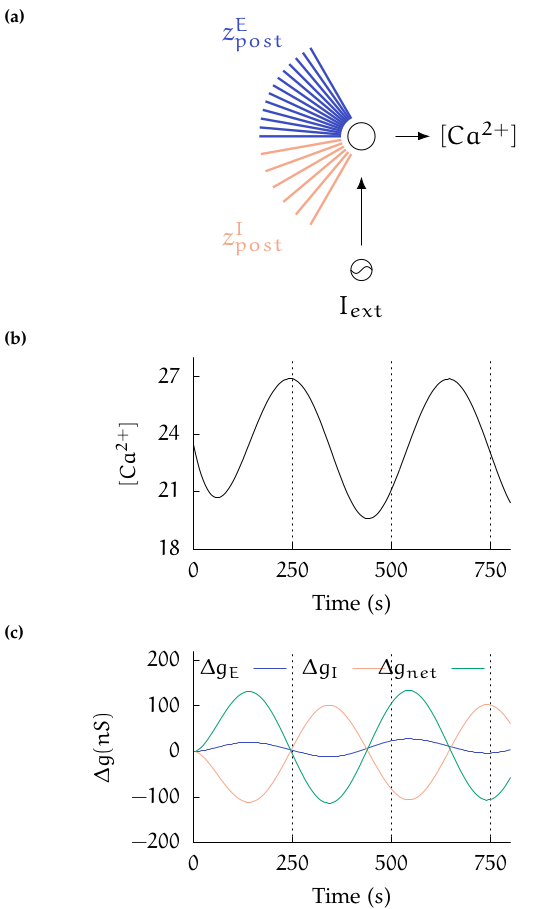
\includegraphics[width=0.4\linewidth]{99_images/single-neuron-results}
  \end{figure}
\end{frame}
\begin{frame}[c]
  \frametitle{New growth curves for pre-synaptic neurites}
  \begin{figure}[h]
  \begin{subfigure}[h]{0.4\textwidth}
    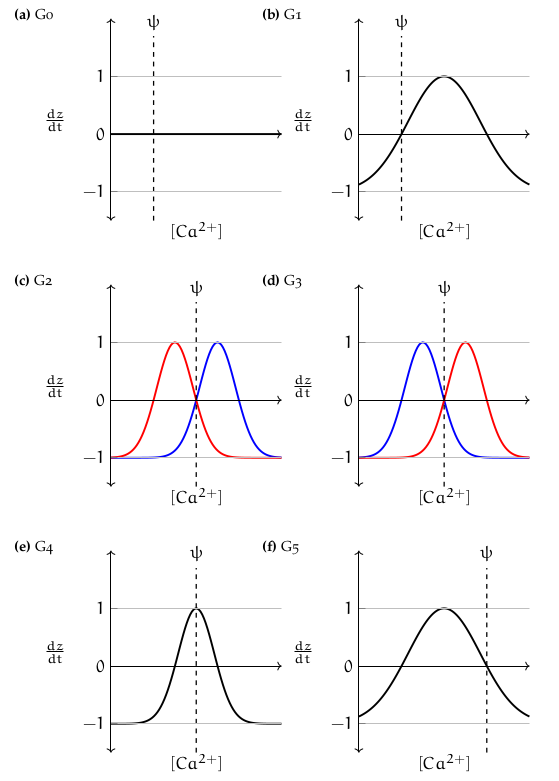
\includegraphics[width=\textwidth]{99_images/possible-growth-pre}
  \end{subfigure}
  \begin{subfigure}[c]{0.5\textwidth}
    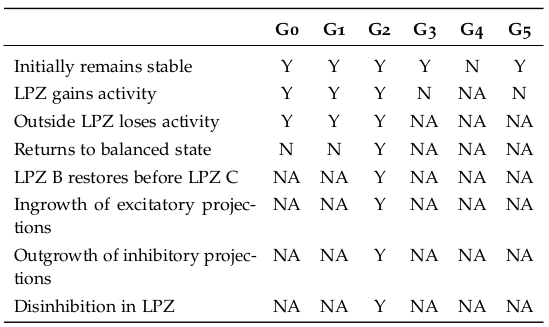
\includegraphics[width=\textwidth]{99_images/growth-pre-table.png}
  \end{subfigure}
  \end{figure}
\end{frame}
\begin{frame}[c]
  \frametitle{New growth curves for pre-synaptic neurites}
  \begin{figure}[h]
    \centering
    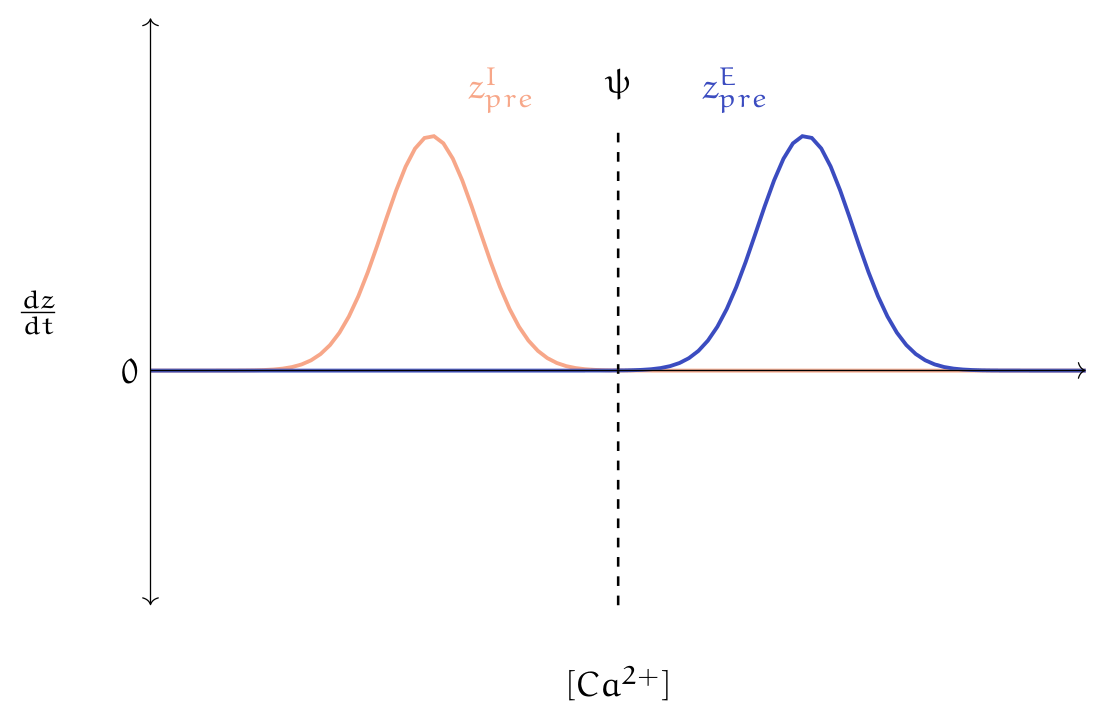
\includegraphics[width=0.6\linewidth]{99_images/growth-pre}
  \end{figure}
\end{frame}
\begin{frame}[c]
  \frametitle{Both synaptic and structural plasticity are necessary for repair}
  \begin{figure}[h]
    \centering
    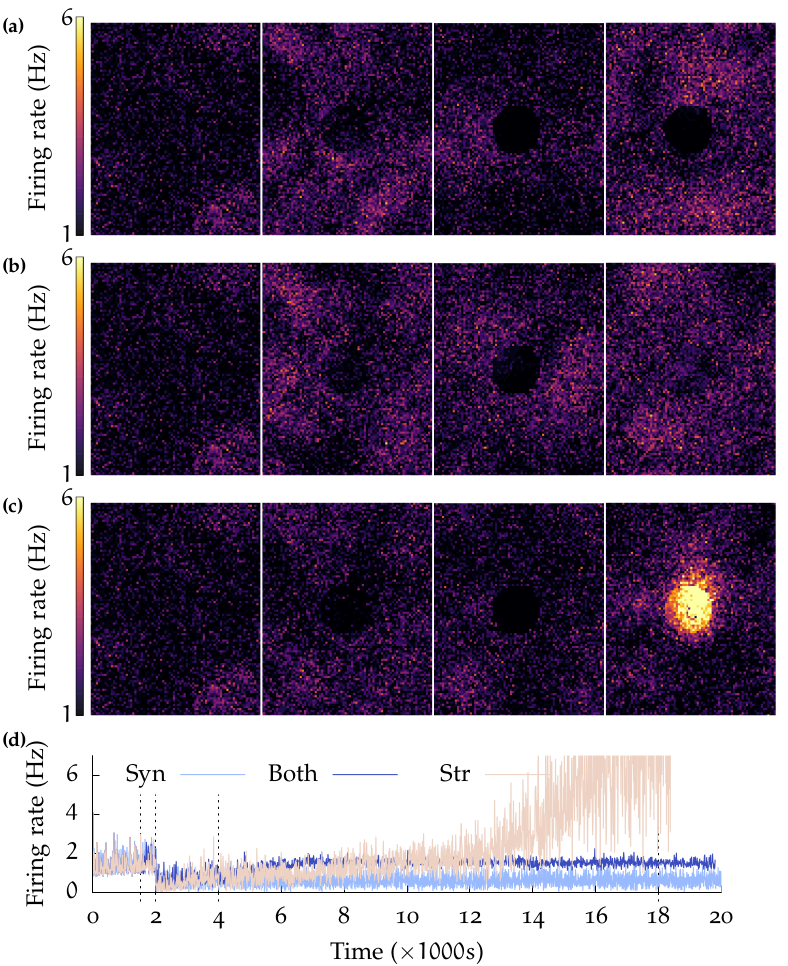
\includegraphics[width=0.6\linewidth]{99_images/syn-str-both}
  \end{figure}
\end{frame}
\begin{frame}[c]
  \frametitle{Associative memory performance after deafferentation (no repair)}
  \begin{figure}[h]
    \centering
    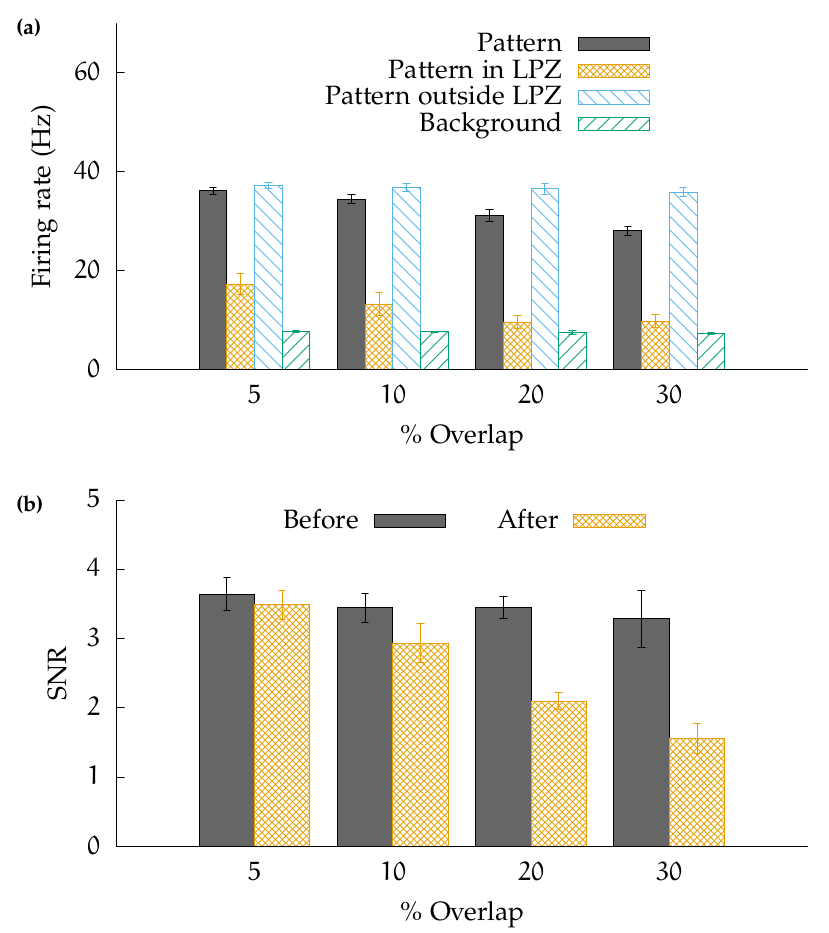
\includegraphics[width=0.6\linewidth]{99_images/performance-deaff-only}
  \end{figure}
\end{frame}
\begin{frame}[c]
  \frametitle{Associative memory performance during repair}
  \begin{figure}[h]
    \centering
    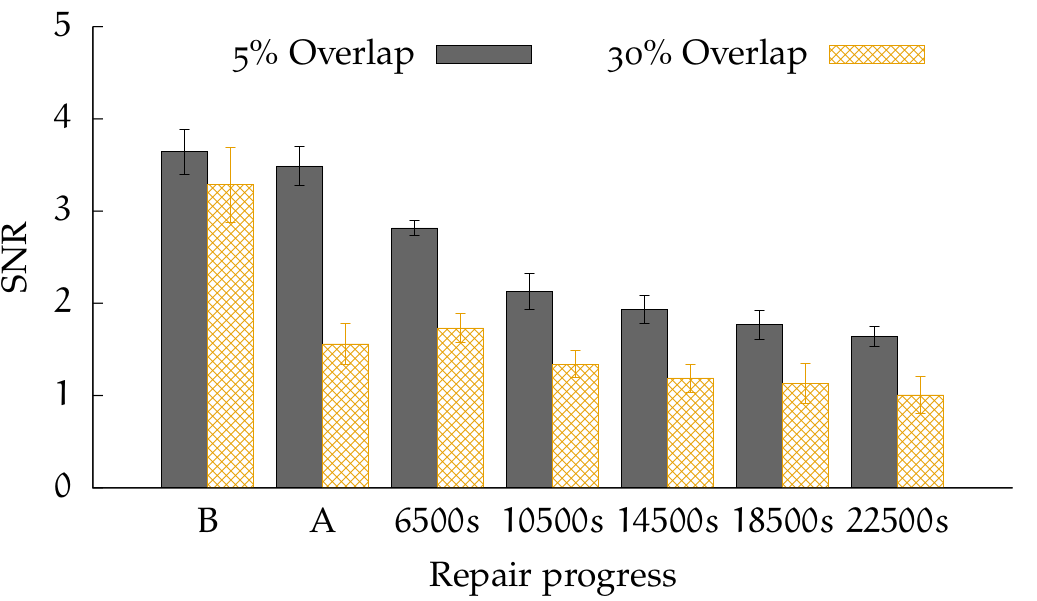
\includegraphics[width=0.6\linewidth]{99_images/performance-during-repair}
  \end{figure}
\end{frame}
\end{document}

